\documentclass{article}
\author{Riccardo Salvalaggio}
\title{ADBIS Exercises}
\usepackage{geometry}
\usepackage{float}
\usepackage{graphicx}
\usepackage{amsmath}
\usepackage{hyperref}
\usepackage{algorithm}
\usepackage{color}
\usepackage[table,xcdraw]{xcolor}
\usepackage{amssymb}
\input{insbox}

\begin{document}
\maketitle
\newpage
\tableofcontents
\newpage


\section{Sheet 1}
\section{Sheet 2}
\section{Sheet 3}
\subsection{Exercise 1}
\begin{itemize}
\item \textbf{a. }
\item \textbf{b. }
without unwind works as well

\end{itemize}

\section{Sheet 4}
\subsection{Exercise 1}
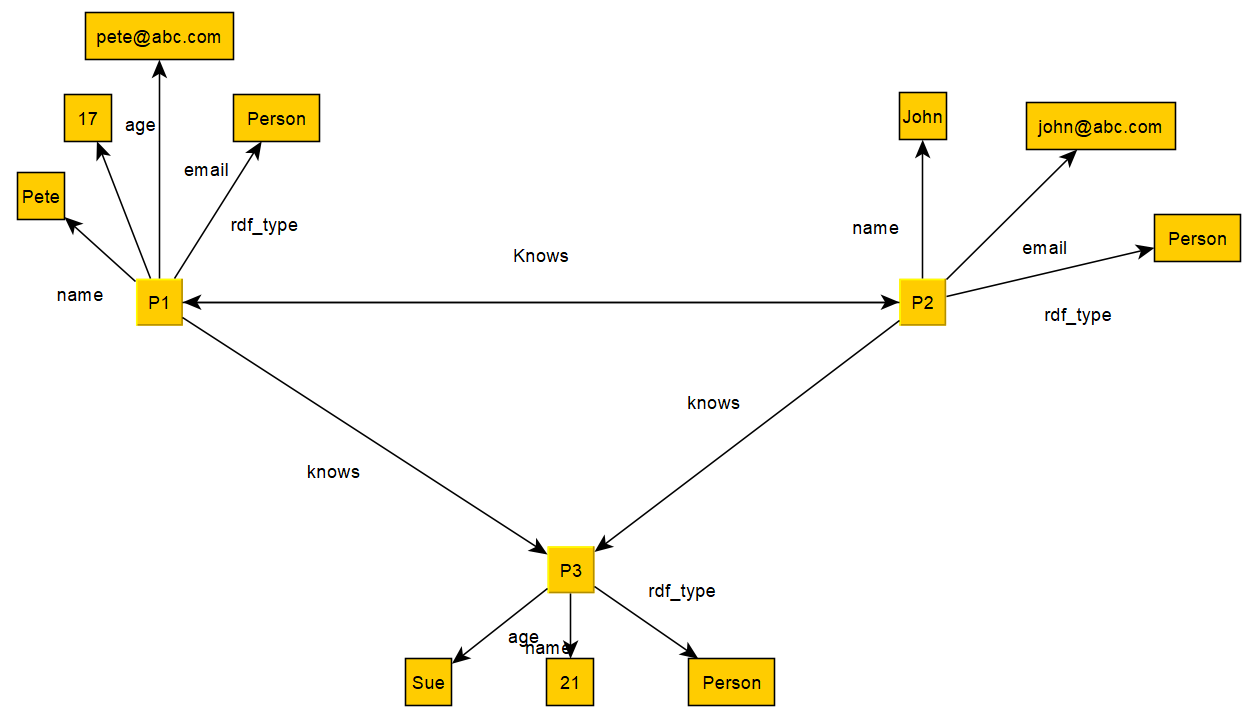
\includegraphics[scale=0.6]{RDF_DB.png}
\begin{itemize}
\item \textbf{a. }Find all the persons with attribute age $>$ 20 and print it.
\item \textbf{b. }Find all the persons with attribute name  and optionally age and print them.
\item \textbf{c. }Find all persons with attribute age and/or their email.
\item \textbf{d. }Find all persons with optionally email without bounds.
\end{itemize}
\subsection{Exercise 2}
\begin{itemize}
\item \textbf{a. } SELECT ?p1 ?p2  \\WHERE $\{$ \\?p1 rdf:type Person.\\ ?p2 rdf:type Person\\  ?p1 knows ?p3 \\ ?p2 knows ?p3 \\ FILTER(?p1 = ?p3)$\}$
\item \textbf{b. } SELECT DISTINCT ?name ?email ?age \\
WHERE { 
?p rdf:type Person .\\
?p name ?name. \\
{ { ?p knows ?p2 } UNION { ?p age ?age2 FILTER (?age2$<$20) } } \\OPTIONAL { ?p email ?email } OPTIONAL { ?p age ?age }}

\item \textbf{c. } SELECT ?p1 ?p2\\ WHERE { \\?p1 knows+ ?p2 FILTER (?p1!=?p2)\\}

\item \textbf{d. } SELECT ?p1 ?p2\\ WHERE { \\?p1 knows+ ?p2 FILTER (?p1!=?p2).\\ ?p2 knows+ ?p1 \\FILTER (?p1!=?p2).\\}
\end{itemize}

\section{Sheet 5: Column Stores and NoSQL}
\subsection{Exercise 5.1: (Column Striping}
Assume you are given the following semi-structured representation of hotels.\\
hotelID : ’h1’\\
hotel :\\
name : ’Palace Hotel’\\
staff :\\
language : ’English’\\
staff :\\
language : ’German’\\
language : ’English’\\
staff :\\
language : ’Spanish’\\
language : ’English’\\
hotelID : ’h2’\\
hotel :\\
name : ’Eden Hotel’\\
address :\\
city : ’Oldtown’\\
roomprice :\\
single : 85\\
double : 120\\
hotelID : ’h3’\\
hotel :\\
name : ’Leonardo Hotel’\\
address :\\
city : ’Newtown’\\
roomprice :\\
double : 100\\
staff :\\
language : ’English’\\
staff :\\
language : ’French’\\\\

\subsubsection{a. Apply the typing for nested records as introduced in the lecture. Try to infer which information is required and which is optional.}
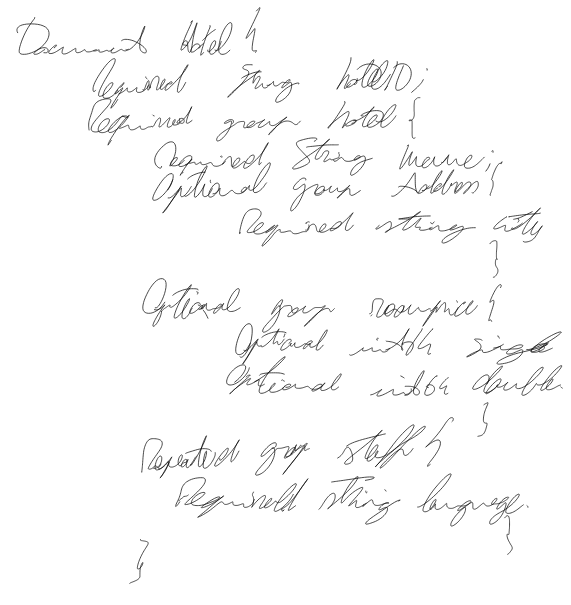
\includegraphics[scale=0.4]{5_1.png}
\subsubsection{b. Write down the document as key-value pairs.}
hotelID : ’h1’\\
hotel.name : ’Palace Hotel’\\
staff.language : ’English’\\
staff.language : ’German’\\
staff.language : ’English’\\
staff.language : ’Spanish’\\
staff.language : ’English’\\\\

hotelID : ’h2’\\
hotel.name : ’Eden Hotel’\\
hotel.address.city : ’Oldtown’\\
hotel.roomprice.single : 85\\
hotel.roomprice.double : 120\\\\

hotelID : ’h3’\\
hotel.name : ’Leonardo Hotel’\\
hotel.address.city : ’Newtown’\\
hotel.roomprice.double : 100\\
staff.language : ’English’\\
staff.language : ’French’\\\\

\subsubsection{c. Add appropriate assignments for repetition- as well as definition levels to the key-value pairs.}

hotelID : ’h1’ (rep: 0,def: 0)\\
hotel.name : ’Palace Hotel’ (rep: 0,def: 0)\\
hotel.roomprice.single : null (rep : 0, def : 0)\\
hotel.roomprice.double : null (rep : 0, def : 0)\\
staff.language : ’English’ (rep: 0,def: 2)\\
staff.language : ’German’ (rep: 1,def: 2)\\
staff.language : ’English’ (rep: 2,def: 2)\\
staff.language : ’Spanish’ (rep: 1,def: 2)\\
staff.language : ’English’ (rep: 2,def: 2)\\\\

hotelID : ’h2’ (rep: 0,def: 0)\\
hotel.name : ’Eden Hotel’ (rep: 0,def: 0)\\
hotel.address.city : ’Oldtown’ (rep: 0,def: 1)\\
hotel.roomprice.single : 85 (rep: 0,def: 2)\\
hotel.roomprice.double : 120 (rep: 0,def: 2)\\
staff.language : null (rep : 0, def : 0)\\\\

hotelID : ’h3’ (rep: 0,def: 0)\\
hotel.name : ’Leonardo Hotel’ (rep: 0,def: 0)\\
hotel.address.city : ’Newtown’(rep: 0,def: 1)\\
hotel.roomprice.single : null (rep: 0, def: 1)\\
hotel.roomprice.double : 100 (rep: 0,def: 2)\\
staff.language : ’English’ (rep: 0,def: 2)\\
staff.language : ’French’ (rep: 1,def: 2)\\\\

\subsubsection{d. Write down the result as striped representation.}
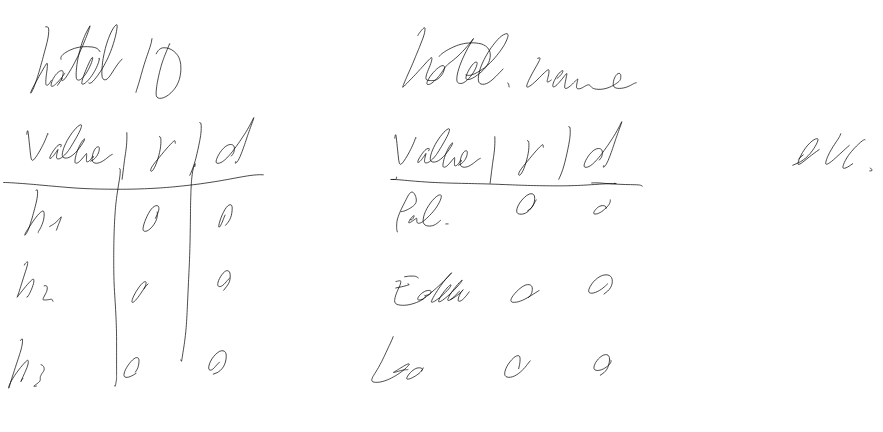
\includegraphics[scale=0.4]{5_4.png}

\subsection{Exercise 5.2: (RDF Storage)}
You are given the following snippet of the mondial RDF graph.\\
@prefix : <http://www.semwebtech.org/mondial/10/meta>.\\
@prefix rdf: <http://www.w3.org/1999/02/22-rdf-syntax-ns>.\\
@prefix xsd: <http://www.w3.org/2001/XMLSchema>.\\
$<$http://www.semwebtech.org/mondial/10/country/AL/$>$ \\
		rdf:type :Country ;\\
		:name "Albania" ;\\
		:carCode ’AL’ ;\\
		:area 28750 ;\\
		:capital $<$http://www.semwebtech.org/mondial/10/country/AL/city/Tirana/$>$.\\
$<$http://www.semwebtech.org/mondial/10/country/GR/$>$ \\
		rdf:type :Country ;\\
		:name "Greece" ;\\
		:area 131940 ;\\
		:capital $<$http://www.semwebtech.org/mondial/10/country/GR/province/Attikis/city/Athina/$>$.\\
$<$http://www.semwebtech.org/mondial/10/country/D/$>$ \\
		rdf:type :Country ;\\
		:name "Germany" ;\\
		:localname "Bundesrepublik Deutschland (die)" ;\\
		:carCode ’D’ ;\\
		:capital $<$http://www.semwebtech.org/mondial/10/country/D/province/Berlin/city/Berlin/$>$.
\subsubsection{a. Encode the graph as triple table.}

\begin{tabular}{ c c c }
 Subject & Predicate & Object \\ 
 country/AL/ & rdf:type & :Country \\  
 country/AL/ & :name & "Albania"   \\
 country/AL/ & :carCode & 'AL'\\
 country/AL/ & :area & 28750\\
 country/AL/ & :capital & "Tirana"\\
\end{tabular}

\subsubsection{b. Encode the graph as property table.}

Same but in horizontal.

\subsubsection{c. Show the tables after applying vertical partioning on the graph.}

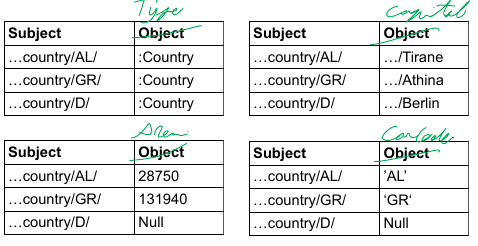
\includegraphics[scale=0.4]{5_7.png}



\section{Sheet 6}
\section{Sheet 7}
\section{Sheet 8}


















\section{Sheet: Conjunctive Query Minimization}
\subsection{Containment and Minimization}
\textbf{Consider the following four Conjunctive Queries, where c denotes a constant.\\
- q1 : ans(X, Y ) $<-$ R(X, A), R(A, B), R(B, Y )\\
- q2 : ans(X, Y ) $<-$ R(X, A), R(A, B), R(B, C), R(C, Y )\\
- q3 : ans(X, Y ) $<-$ R(X, A), R(B, C), R(D, Y ), R(X, B), R(A, C), R(C, Y )\\
- q4 : ans(X, Y ) $<-$ R(X, A), R(A, c), R(c, B), R(B, Y )\\
a) Find all equivalences and containment relationships between the above queries.\\
b) Minimize all queries.}\\\\
\textbf{- Answers: }\\
\textbf{a)}\\
Although $q_4$ looks like $q_2$ , there is no constant c in $q_2$. A constant can never be mapped onto a variable, i.e. $q_2 \nsubseteq q_4$. Conversely, however, $q_4 \sqsubseteq q_2$ (the containment mapping maps B to constant c, C to B and all other variables to itself).\\
Furthermore, $q_1 \nsubseteq q_2$, $q_2 \nsubseteq q_1$ and $q_1 \equiv q_3$ hold (the latter equivalence will be shown in the second part of the task).\\
\textbf{b)}\\
$q_1 , q_2$ and $q_4$ are already minimised. Minimisation of $q_3$:\\
ans(X,Y) $<-$ R(X,A), R(B,C), R(D,Y), R(X,B), R(A,C), R(C,Y);\\
ans(U,V) $<-$ R(U,W), R(P,L), R(N,V), R(U,P), R(W,L), R(L,V);\\
\textbf{Figure:}\\
$\theta$ : {U $->$ X, V $->$ Y, W $->$ A, P $->$ A, L $->$ C, N $->$ D}\\
After removing R(B,C) and R(X,B), we obtain $q_3'$:\\
ans(X,Y) $<-$ R(X,A), R(A,C), R(D,Y), R(C,Y), which can be rewritten:\\
ans(U,V) $<-$ R(U,W), R(W,T), R(P,V), R(T,V) and minimised:\\
$\theta$: {U $->$ X, V $->$ Y, W $->$ A, T $->$ C, P $->$ C}\\
to the query ans(X,Y) $<-$ R(X,A), R(A,C), R(C,Y) which is equivalent to $q_1$ .\\
$q_3 \equiv q_1$.\\
\textbf{Alternative mapping:}\\
$\theta$ : {U $->$ X, V $->$ Y, W $->$ A, P $->$ A, L $->$ C, N $->$ C}\\
ans(X, Y) $<-$ R(X,A), R(A,C), R(C,Y) $\rightarrow$ $q_3 \equiv q_1$.\\

\subsection{CQ Minimization}
\textbf{Instead of eliminating subgoals, query minimization can also be achieved by eliminating variables. Write an algorithm which minimizes queries by eliminating each time at least one variable. Prove that your algorithm generates a minimal query.\\\\}
\textbf{- Answer:}\\
The minimization algorithm by removing the variables works analogously to the one by removing subgoals. It involves a stepwise picking a variable v from the current CQ Q, and find a containment mapping $\rho$ from V to V$/$v,  such that for each subgoal Ri ( Vi ), $\rho$(Ri(Vi )) can be found in the body of Q. If this is the case, then we can remove all the subgoals containing v. Otherwise the algorithm stops.\\
To show the removing of variables is equivalent to removing of subgoals, we have to prove:\\ \textbf{1.} If one variable can be removed, then there is at least one subgoal which can be removed.\\ This is obvious from the algorithm. \\
\textbf{2.} If one subgoal can be removed, then there is at least one variable can be removed as well. \\
To show this, assume we have found a subgoal Ri (Vi ), which can be removed. This means there is a containment mapping $rho$ from the variables from the CQ Q to the variables to Q, such that $\rho$(Ri ( Vi )) is mapped to another subgoal other than itself. This means, $rho$ maps at least one variable v $\in$ Vi to some other variable v0 in Q. If $rho$ maps some other variable v00 to v, then we can simply change the mapping from
v00 $->$ v to v 00 $->$ v 0 , so that the containment holds as well. So we have constructed a new containment mapping from V to V \ v. Thus we could remove v accordingly.

\subsection{Acyclic CQ}
q(X, T ) $<-$ R1(X, Y, Z), R2(Y, V ), R3(Y, Z, U ), R4(Z, U, W ), R5(U, W, T ).\\
q(X, W ) $<-$ R1(X, Y, Z), R3(Y, Z, U ), R4(Z, U, W ), R5(U, W, X).






























\section{Sheet: Conjunctive Query Minimization}
\subsection{Acyclic CQ}
\textbf{Given the following CQ with the database instance R(1, 2, 3), R(2, 3, 4), R(3, 4, 5), R(4, 5, 6), S(3, 8), S(4, 9).\\
q(X, T ) $\leftarrow$ R(X, Y, Z), S(Y, V ), R(Y, Z, U ), R(Z, U, T ), R(X, Y, W ).\\
a) Apply GYO Algorithm to show the query is acyclic.\\
b) Give the join tree of the query.\\
c) Apply the semi-join algorithm over the join tree on the given database and obtain the query answer.\\\\}
\textbf{- Answers:}
q(X,T) $\leftarrow$ R(X,Y,Z) $\wedge$ S(Y,V) $\wedge$ R(Y,Z,U) $\wedge$ R(Z,U,T) $\wedge$ R(X,Y,W).
\begin{itemize}
\item \textbf{a)}\\\\
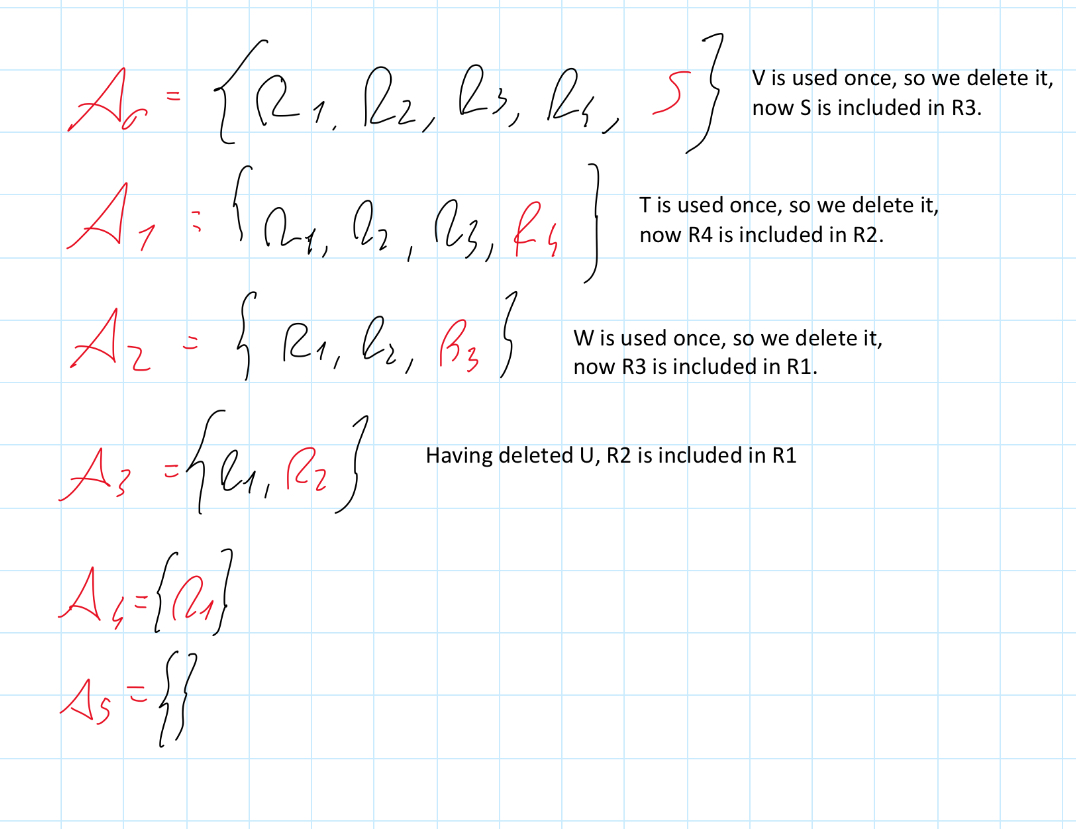
\includegraphics[scale=0.2]{10_1.jpg}
\item \textbf{b}\\\\
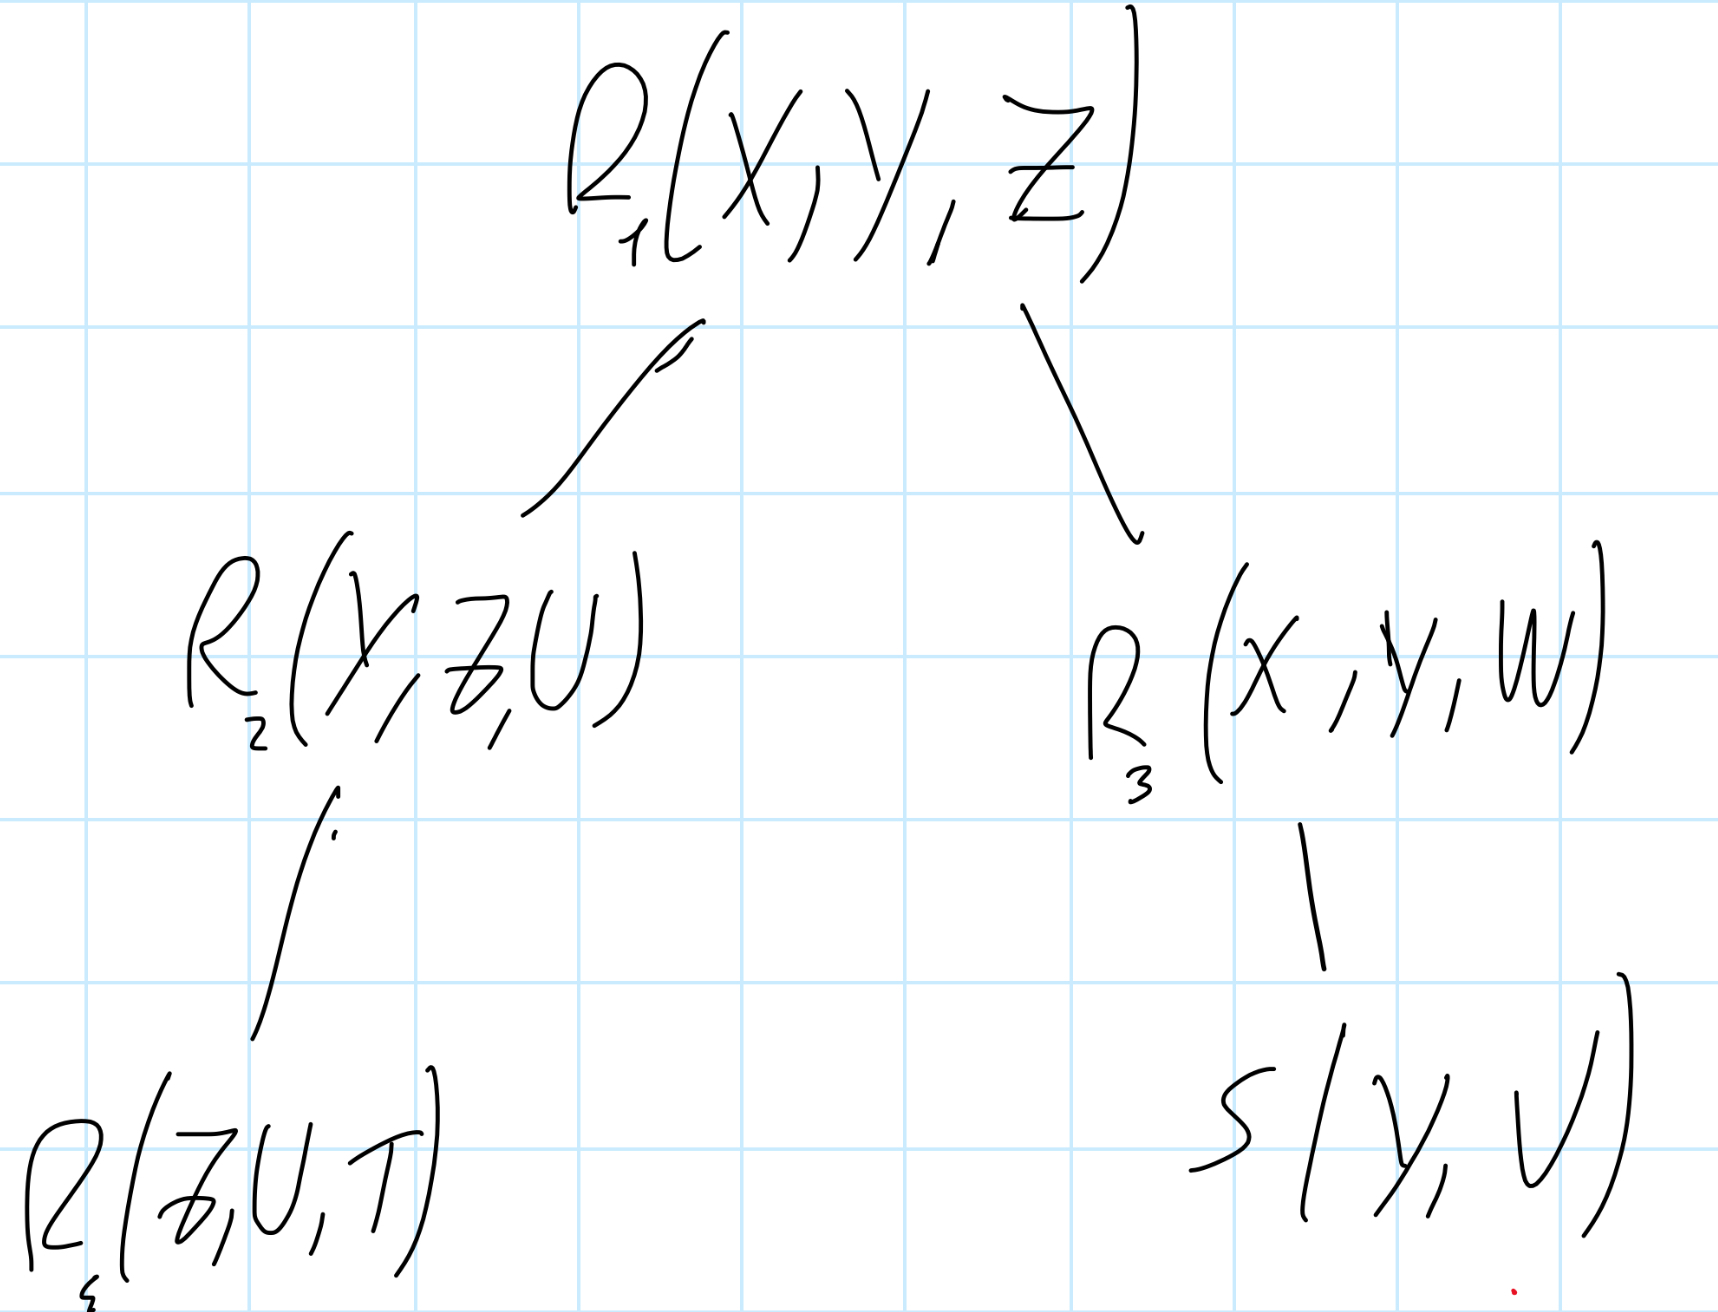
\includegraphics[scale=0.1]{10_2.jpg}
\item \textbf{c}\\\\
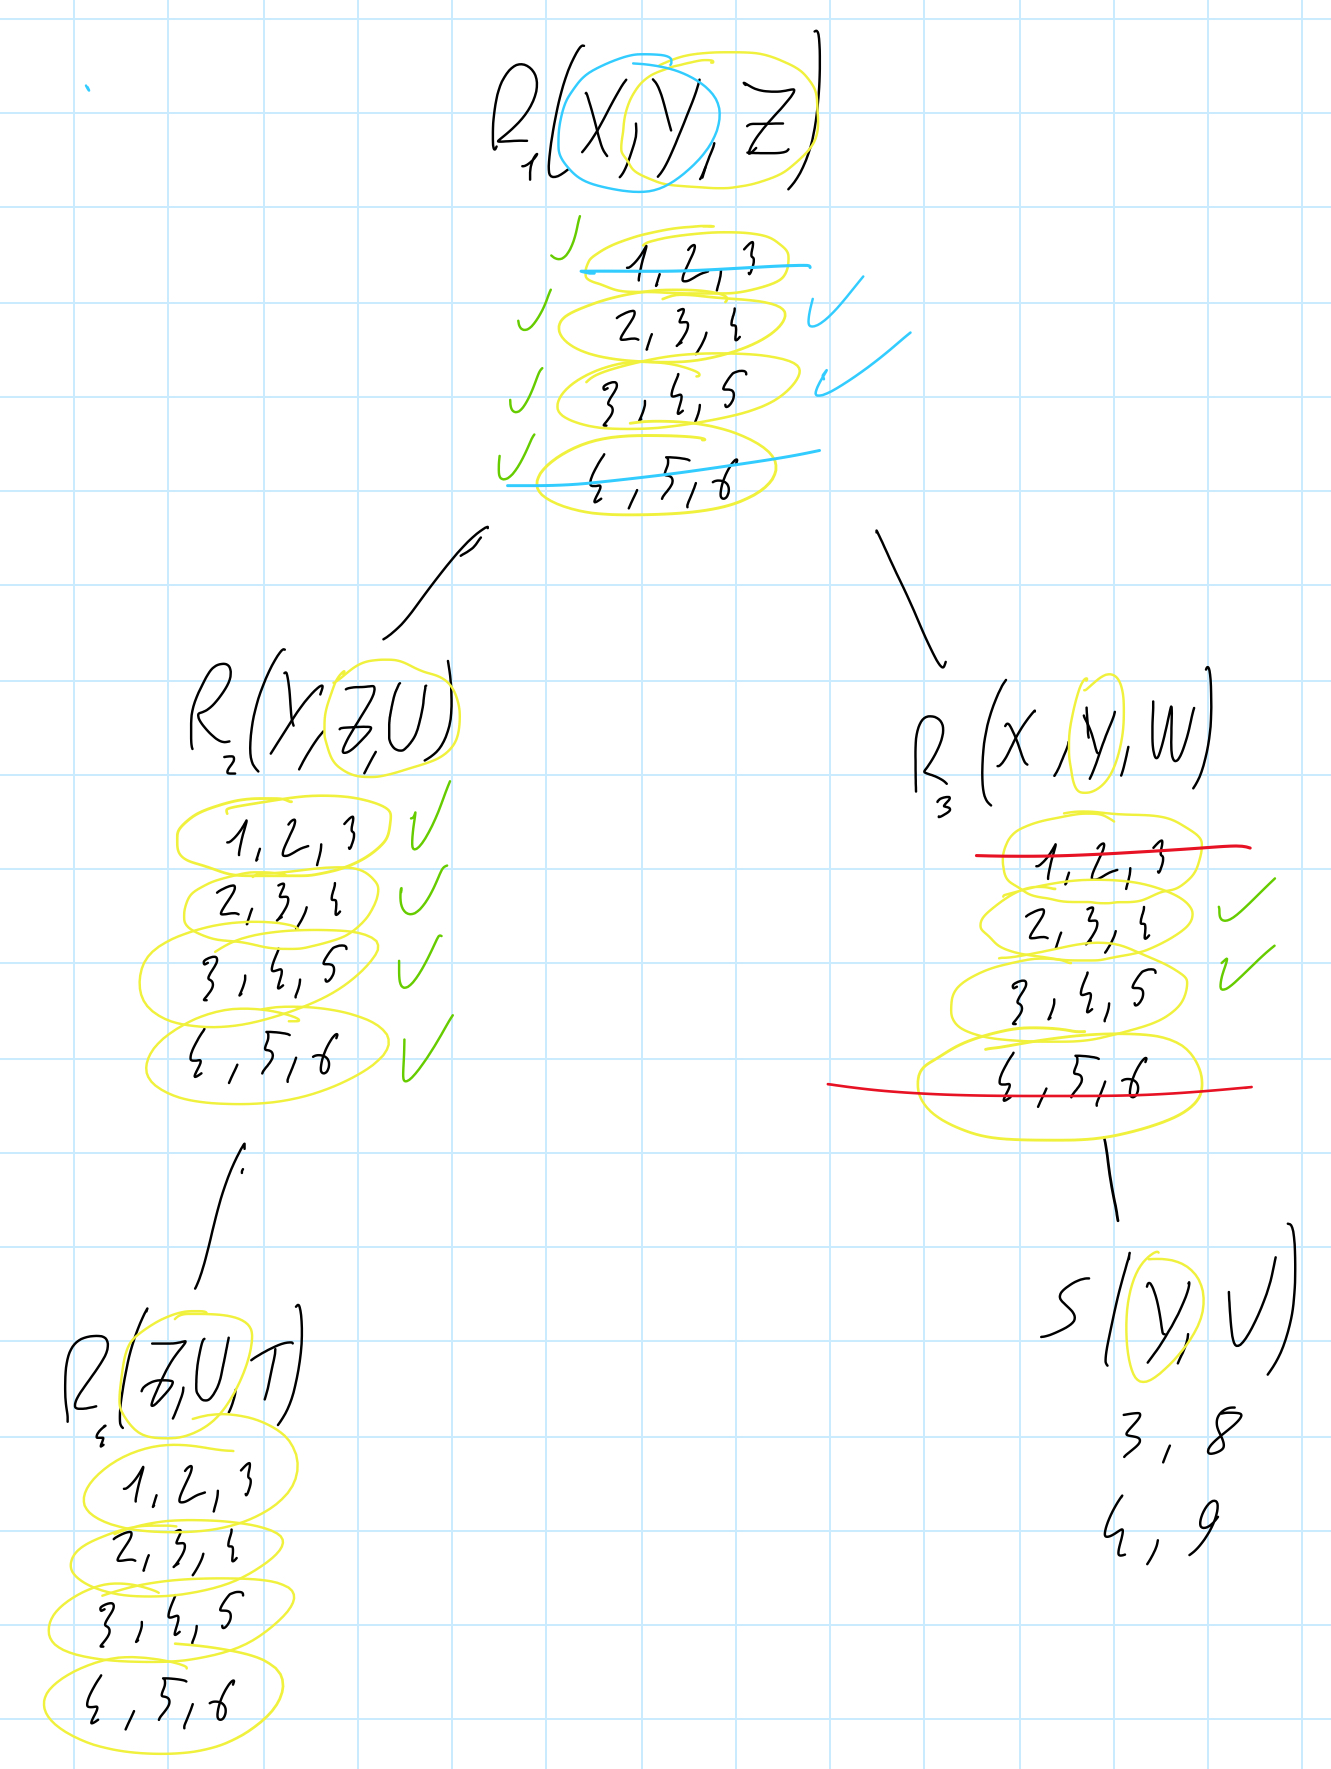
\includegraphics[scale=0.2]{10_3.jpg}\\\\
q(X,T) $\rightarrow$ (2,4),(3,5)
\end{itemize}

\subsection{Datalog}
\textbf{Consider a directed graph which is given by E(X, Y ) (edges). Give a Datalog program which computes the following relations:\\
a) Odd(X, Y ), which holds if there is a path with odd length from X to Y .\\
b) Oddcycle(X), there is a cycle with odd length through X.\\
c) Evencycle(X), there is cycle with even length through X.\\
d) Bothcycles(X), there are cycles with even length and cycles with odd length through X.}\\\\
\textbf{- Answers:}\\
\textit{\textbf{a)} Odd(X,Y): }\\
   Odd(X,Y) = E(X,Y).\\
   Even(X,Y) = Odd(X,Y),Odd(Y,Z).\\
   Odd(X,Y) = Odd(X,Z),Even(Z,Y).\\
\textit{\textbf{b)} Oddcycle(X):  }\\
   Oddcycle(X) = Odd(X,X)\\
\textit{\textbf{c)} Evencycle(X): }\\
   Evencycle(X) = Even(X,X).\\
\textit{d) Bothcycles(X):}\\
Botchcycles(X) = Oddcycle(X), Evencycle(X).

\subsection{Datalog}
\textbf{parent(X, Y ) is a family tree with root p. Please give a Datalog program, which computes the predicates: a) samegeneration(X, Y ), b) sibling(X, Y ) and c) cousin(X, Y ). (samegeneration(X, Y ) holds, if the distance between X and p is the same as the distance between Y and p; sibling(X, Y ) is true, if X and Y have the same parent; cousin(X, Y ) holds, if X and Y belong to the same generation but are not siblings).
Hint: You may use negation in your programs.}\\\\
\textbf{- Answers:}\\
\textit{\textbf{a): }}\\
SameGeneration(X,Y) $\leftarrow$ Siblings(X,Y)\\
SameGeneration(X,Y) $\leftarrow$ Parent(W,X),Parent(Z,Y), SameGeneration(W,Z)\\
\textit{\textbf{b): }}\\
Siblings(X,Y) $\leftarrow$ Parent(Z,X),Parent(Z,Y)\\
\textit{\textbf{c): }}\\
Cousins(X,Y) $\leftarrow$ SameGeneration(X,Y),$\neg$Siblings(X,Y)





\end{document}